
%% bare_conf.tex
%% V1.4
%% 2012/12/27
%% by Michael Shell
%% See:
%% http://www.michaelshell.org/
%% for current contact information.
%%
%% This is a skeleton file demonstrating the use of IEEEtran.cls
%% (requires IEEEtran.cls version 1.8 or later) with an IEEE conference paper.
%%
%% Support sites:
%% http://www.michaelshell.org/tex/ieeetran/
%% http://www.ctan.org/tex-archive/macros/latex/contrib/IEEEtran/
%% and
%% http://www.ieee.org/

%%*************************************************************************
%% Legal Notice:
%% This code is offered as-is without any warranty either expressed or
%% implied; without even the implied warranty of MERCHANTABILITY or
%% FITNESS FOR A PARTICULAR PURPOSE!
%% User assumes all risk.
%% In no event shall IEEE or any contributor to this code be liable for
%% any damages or losses, including, but not limited to, incidental,
%% consequential, or any other damages, resulting from the use or misuse
%% of any information contained here.
%%
%% All comments are the opinions of their respective authors and are not
%% necessarily endorsed by the IEEE.
%%
%% This work is distributed under the LaTeX Project Public License (LPPL)
%% ( http://www.latex-project.org/ ) version 1.3, and may be freely used,
%% distributed and modified. A copy of the LPPL, version 1.3, is included
%% in the base LaTeX documentation of all distributions of LaTeX released
%% 2003/12/01 or later.
%% Retain all contribution notices and credits.
%% ** Modified files should be clearly indicated as such, including  **
%% ** renaming them and changing author support contact information. **
%%
%% File list of work: IEEEtran.cls, IEEEtran_HOWTO.pdf, bare_adv.tex,
%%                    bare_conf.tex, bare_jrnl.tex, bare_jrnl_compsoc.tex,
%%                    bare_jrnl_transmag.tex
%%*************************************************************************

% *** Authors should verify (and, if needed, correct) their LaTeX system  ***
% *** with the testflow diagnostic prior to trusting their LaTeX platform ***
% *** with production work. IEEE's font choices can trigger bugs that do  ***
% *** not appear when using other class files.                            ***
% The testflow support page is at:
% http://www.michaelshell.org/tex/testflow/



% Note that the a4paper option is mainly intended so that authors in
% countries using A4 can easily print to A4 and see how their papers will
% look in print - the typesetting of the document will not typically be
% affected with changes in paper size (but the bottom and side margins will).
% Use the testflow package mentioned above to verify correct handling of
% both paper sizes by the user's LaTeX system.
%
% Also note that the "draftcls" or "draftclsnofoot", not "draft", option
% should be used if it is desired that the figures are to be displayed in
% draft mode.
%
\documentclass[conference]{IEEEtran}
% Add the compsoc option for Computer Society conferences.
%
% If IEEEtran.cls has not been installed into the LaTeX system files,
% manually specify the path to it like:
% \documentclass[conference]{../sty/IEEEtran}





% Some very useful LaTeX packages include:
% (uncomment the ones you want to load)


% *** MISC UTILITY PACKAGES ***
%
%\usepackage{ifpdf}
% Heiko Oberdiek's ifpdf.sty is very useful if you need conditional
% compilation based on whether the output is pdf or dvi.
% usage:
% \ifpdf
%   % pdf code
% \else
%   % dvi code
% \fi
% The latest version of ifpdf.sty can be obtained from:
% http://www.ctan.org/tex-archive/macros/latex/contrib/oberdiek/
% Also, note that IEEEtran.cls V1.7 and later provides a builtin
% \ifCLASSINFOpdf conditional that works the same way.
% When switching from latex to pdflatex and vice-versa, the compiler may
% have to be run twice to clear warning/error messages.





% *** CITATION PACKAGES ***
%
\usepackage{cite}
% cite.sty was written by Donald Arseneau
% V1.6 and later of IEEEtran pre-defines the format of the cite.sty package
% \cite{} output to follow that of IEEE. Loading the cite package will
% result in citation numbers being automatically sorted and properly
% "compressed/ranged". e.g., [1], [9], [2], [7], [5], [6] without using
% cite.sty will become [1], [2], [5]--[7], [9] using cite.sty. cite.sty's
% \cite will automatically add leading space, if needed. Use cite.sty's
% noadjust option (cite.sty V3.8 and later) if you want to turn this off
% such as if a citation ever needs to be enclosed in parenthesis.
% cite.sty is already installed on most LaTeX systems. Be sure and use
% version 4.0 (2003-05-27) and later if using hyperref.sty. cite.sty does
% not currently provide for hyperlinked citations.
% The latest version can be obtained at:
% http://www.ctan.org/tex-archive/macros/latex/contrib/cite/
% The documentation is contained in the cite.sty file itself.






% *** GRAPHICS RELATED PACKAGES ***
%
\ifCLASSINFOpdf
  \usepackage[pdftex]{graphicx}
  \usepackage{epstopdf}
  % declare the path(s) where your graphic files are
  % \graphicspath{{../pdf/}{../jpeg/}}
  % and their extensions so you won't have to specify these with
  % every instance of \includegraphics
  % \DeclareGraphicsExtensions{.pdf,.jpeg,.png}
\else
  % or other class option (dvipsone, dvipdf, if not using dvips). graphicx
  % will default to the driver specified in the system graphics.cfg if no
  % driver is specified.
  % \usepackage[dvips]{graphicx}
  % declare the path(s) where your graphic files are
  % \graphicspath{{../eps/}}
  % and their extensions so you won't have to specify these with
  % every instance of \includegraphics
  % \DeclareGraphicsExtensions{.eps}
\fi
% graphicx was written by David Carlisle and Sebastian Rahtz. It is
% required if you want graphics, photos, etc. graphicx.sty is already
% installed on most LaTeX systems. The latest version and documentation
% can be obtained at:
% http://www.ctan.org/tex-archive/macros/latex/required/graphics/
% Another good source of documentation is "Using Imported Graphics in
% LaTeX2e" by Keith Reckdahl which can be found at:
% http://www.ctan.org/tex-archive/info/epslatex/
%
% latex, and pdflatex in dvi mode, support graphics in encapsulated
% postscript (.eps) format. pdflatex in pdf mode supports graphics
% in .pdf, .jpeg, .png and .mps (metapost) formats. Users should ensure
% that all non-photo figures use a vector format (.eps, .pdf, .mps) and
% not a bitmapped formats (.jpeg, .png). IEEE frowns on bitmapped formats
% which can result in "jaggedy"/blurry rendering of lines and letters as
% well as large increases in file sizes.
%
% You can find documentation about the pdfTeX application at:
% http://www.tug.org/applications/pdftex





% *** MATH PACKAGES ***
%
\usepackage[cmex10]{amsmath}
% A popular package from the American Mathematical Society that provides
% many useful and powerful commands for dealing with mathematics. If using
% it, be sure to load this package with the cmex10 option to ensure that
% only type 1 fonts will utilized at all point sizes. Without this option,
% it is possible that some math symbols, particularly those within
% footnotes, will be rendered in bitmap form which will result in a
% document that can not be IEEE Xplore compliant!
%
% Also, note that the amsmath package sets \interdisplaylinepenalty to 10000
% thus preventing page breaks from occurring within multiline equations. Use:
%\interdisplaylinepenalty=2500
% after loading amsmath to restore such page breaks as IEEEtran.cls normally
% does. amsmath.sty is already installed on most LaTeX systems. The latest
% version and documentation can be obtained at:
% http://www.ctan.org/tex-archive/macros/latex/required/amslatex/math/





% *** SPECIALIZED LIST PACKAGES ***
\usepackage{algorithm}
\usepackage{algorithmic}
% algorithmic.sty was written by Peter Williams and Rogerio Brito.
% This package provides an algorithmic environment fo describing algorithms.
% You can use the algorithmic environment in-text or within a figure
% environment to provide for a floating algorithm. Do NOT use the algorithm
% floating environment provided by algorithm.sty (by the same authors) or
% algorithm2e.sty (by Christophe Fiorio) as IEEE does not use dedicated
% algorithm float types and packages that provide these will not provide
% correct IEEE style captions. The latest version and documentation of
% algorithmic.sty can be obtained at:
% http://www.ctan.org/tex-archive/macros/latex/contrib/algorithms/
% There is also a support site at:
% http://algorithms.berlios.de/index.html
% Also of interest may be the (relatively newer and more customizable)
% algorithmicx.sty package by Szasz Janos:
% http://www.ctan.org/tex-archive/macros/latex/contrib/algorithmicx/




% *** ALIGNMENT PACKAGES ***
%
\usepackage{array}
% Frank Mittelbach's and David Carlisle's array.sty patches and improves
% the standard LaTeX2e array and tabular environments to provide better
% appearance and additional user controls. As the default LaTeX2e table
% generation code is lacking to the point of almost being broken with
% respect to the quality of the end results, all users are strongly
% advised to use an enhanced (at the very least that provided by array.sty)
% set of table tools. array.sty is already installed on most systems. The
% latest version and documentation can be obtained at:
% http://www.ctan.org/tex-archive/macros/latex/required/tools/


% IEEEtran contains the IEEEeqnarray family of commands that can be used to
% generate multiline equations as well as matrices, tables, etc., of high
% quality.




% *** SUBFIGURE PACKAGES ***
%\ifCLASSOPTIONcompsoc
%  \usepackage[caption=false,font=normalsize,labelfont=sf,textfont=sf]{subfig}
%\else
%  \usepackage[caption=false,font=footnotesize]{subfig}
%\fi
% subfig.sty, written by Steven Douglas Cochran, is the modern replacement
% for subfigure.sty, the latter of which is no longer maintained and is
% incompatible with some LaTeX packages including fixltx2e. However,
% subfig.sty requires and automatically loads Axel Sommerfeldt's caption.sty
% which will override IEEEtran.cls' handling of captions and this will result
% in non-IEEE style figure/table captions. To prevent this problem, be sure
% and invoke subfig.sty's "caption=false" package option (available since
% subfig.sty version 1.3, 2005/06/28) as this is will preserve IEEEtran.cls
% handling of captions.
% Note that the Computer Society format requires a larger sans serif font
% than the serif footnote size font used in traditional IEEE formatting
% and thus the need to invoke different subfig.sty package options depending
% on whether compsoc mode has been enabled.
%
% The latest version and documentation of subfig.sty can be obtained at:
% http://www.ctan.org/tex-archive/macros/latex/contrib/subfig/




% *** FLOAT PACKAGES ***
%
%\usepackage{fixltx2e}
% fixltx2e, the successor to the earlier fix2col.sty, was written by
% Frank Mittelbach and David Carlisle. This package corrects a few problems
% in the LaTeX2e kernel, the most notable of which is that in current
% LaTeX2e releases, the ordering of single and double column floats is not
% guaranteed to be preserved. Thus, an unpatched LaTeX2e can allow a
% single column figure to be placed prior to an earlier double column
% figure. The latest version and documentation can be found at:
% http://www.ctan.org/tex-archive/macros/latex/base/


%\usepackage{stfloats}
% stfloats.sty was written by Sigitas Tolusis. This package gives LaTeX2e
% the ability to do double column floats at the bottom of the page as well
% as the top. (e.g., "\begin{figure*}[!b]" is not normally possible in
% LaTeX2e). It also provides a command:
%\fnbelowfloat
% to enable the placement of footnotes below bottom floats (the standard
% LaTeX2e kernel puts them above bottom floats). This is an invasive package
% which rewrites many portions of the LaTeX2e float routines. It may not work
% with other packages that modify the LaTeX2e float routines. The latest
% version and documentation can be obtained at:
% http://www.ctan.org/tex-archive/macros/latex/contrib/sttools/
% Do not use the stfloats baselinefloat ability as IEEE does not allow
% \baselineskip to stretch. Authors submitting work to the IEEE should note
% that IEEE rarely uses double column equations and that authors should try
% to avoid such use. Do not be tempted to use the cuted.sty or midfloat.sty
% packages (also by Sigitas Tolusis) as IEEE does not format its papers in
% such ways.
% Do not attempt to use stfloats with fixltx2e as they are incompatible.
% Instead, use Morten Hogholm'a dblfloatfix which combines the features
% of both fixltx2e and stfloats:
%
% \usepackage{dblfloatfix}
% The latest version can be found at:
% http://www.ctan.org/tex-archive/macros/latex/contrib/dblfloatfix/




% *** PDF, URL AND HYPERLINK PACKAGES ***
%
%\usepackage{url}
% url.sty was written by Donald Arseneau. It provides better support for
% handling and breaking URLs. url.sty is already installed on most LaTeX
% systems. The latest version and documentation can be obtained at:
% http://www.ctan.org/tex-archive/macros/latex/contrib/url/
% Basically, \url{my_url_here}.




% *** Do not adjust lengths that control margins, column widths, etc. ***
% *** Do not use packages that alter fonts (such as pslatex).         ***
% There should be no need to do such things with IEEEtran.cls V1.6 and later.
% (Unless specifically asked to do so by the journal or conference you plan
% to submit to, of course. )


% correct bad hyphenation here
\hyphenation{op-tical net-works semi-conduc-tor}


\begin{document}
%
% paper title
% can use linebreaks \\ within to get better formatting as desired
% Do not put math or special symbols in the title.
\title{A Novel Link Scheduling Algorithm for Wireless Networks using Directional Antenna}


% author names and affiliations
% use a multiple column layout for up to three different
% affiliations

\author{\IEEEauthorblockN{Zhaoshu Tang, Ming Zhu, Lei Wang, Honglian Ma}
\IEEEauthorblockA{School of Software\\
Dalian University of Technology, China\\
tang.zhaoshu@mail.dlut.edu.cn, zhuming@dlut.edu.cn, lei.wang@dlut.edu.cn, mhl@dlut.edu.cn}
}
% conference papers do not typically use \thanks and this command
% is locked out in conference mode. If really needed, such as for
% the acknowledgment of grants, issue a \IEEEoverridecommandlockouts
% after \documentclass

% for over three affiliations, or if they all won't fit within the width
% of the page, use this alternative format:
%
%\author{\IEEEauthorblockN{Michael Shell\IEEEauthorrefmark{1},
%Homer Simpson\IEEEauthorrefmark{2},
%James Kirk\IEEEauthorrefmark{3},
%Montgomery Scott\IEEEauthorrefmark{3} and
%Eldon Tyrell\IEEEauthorrefmark{4}}
%\IEEEauthorblockA{\IEEEauthorrefmark{1}School of Electrical and Computer Engineering\\
%Georgia Institute of Technology,
%Atlanta, Georgia 30332--0250\\ Email: see http://www.michaelshell.org/contact.html}
%\IEEEauthorblockA{\IEEEauthorrefmark{2}Twentieth Century Fox, Springfield, USA\\
%Email: homer@thesimpsons.com}
%\IEEEauthorblockA{\IEEEauthorrefmark{3}Starfleet Academy, San Francisco, California 96678-2391\\
%Telephone: (800) 555--1212, Fax: (888) 555--1212}
%\IEEEauthorblockA{\IEEEauthorrefmark{4}Tyrell Inc., 123 Replicant Street, Los Angeles, California 90210--4321}}




% use for special paper notices
%\IEEEspecialpapernotice{(Invited Paper)}




% make the title area
\maketitle

% As a general rule, do not put math, special symbols or citations
% in the abstract
\begin{abstract}
For a given set of communication links whose senders transmit at a fixed power level, it is a hot problem to select a maximum set of links that can be transmitted simultaneously, which is known to be NP-hard. The existing algorithm only apply to the condition of omnidirectional transmission. This paper addresses the problem in a plane wireless network where the nodes use directional antennas under physical interference model. We develop a directional interference model applicable to such networks, and first propose the approximation algorithm to solve scheduling problem under this model. We proved the correctness of the algorithm by mathematical analysis. We have also proved the great advantages of using directional antenna by extensive simulations.
\end{abstract}

% no keywords

\begin{IEEEkeywords}
Link Scheduling, Directional Antennas, Physical Interference Model
\end{IEEEkeywords}


% For peer review papers, you can put extra information on the cover
% page as needed:
% \ifCLASSOPTIONpeerreview
% \begin{center} \bfseries EDICS Category: 3-BBND \end{center}
% \fi
%
% For peerreview papers, this IEEEtran command inserts a page break and
% creates the second title. It will be ignored for other modes.
\IEEEpeerreviewmaketitle



\section{Introduction}
% no \IEEEPARstart
This paper mainly studies a typical question in wireless networking which transmit node equip with directional antennas. One of key problem in a given wireless network is to improve the throughput capacity. In the case of shared only one channel, a plurality of communication links transmission at the same time will lead to signal interference. In wireless network, link scheduling problem is to reduce the maximum interference when the links transmit simultaneously, and ensure the message can be successfully accepted by the receiving node. The main objective is to achieve efficient spatial reuse and increase network capacity, considering wireless interference among concurrently transmitting nodes.

By concentrating the energy in specific direction, opposed to omni-directional transmission, Directional antennas can provide the benefits of increased range, reduced interference and increased spatial reuse of bandwidth. Due to the benefits from the directional antennas, the scheduling scheme need to take into account the nature of the antenna beam direction at each node.


The problem \emph{One-slot Maximum Set of Links} (OSML) is to seek a largest set of solution links from a given set $A$ that can be transmitted simultaneously. This optimization problem is NP-hard proved by Gussevskaia \cite{1}. Plenty of research to this problem, some approximation scheduling algorithms was be proposed \cite{1,2}, which is performance good.


Nowadays, various ways to solve the problem of OSML under physical interference model was present. The author of \cite{1} designed the first non-trivial approximation algorithm with approximation bound $O(\log {\frac{\max_{l \in A }d(l)}{\min_{l \in A} d(l)}}) $. Goussevskaia made huge efforts on developing a constant approximation bound in the literature\cite{2}, which proposed a $O(\log {n})$ approximation for the problem of maximizing the number of links scheduled in one time-slot. Then, Peng-Jun Wan $et$ $al$., \cite{3} given a further analysis to the OSML problem under physical interference model. Besides, they summarize the method to solve this kind of problem in\cite{7}. Recently, more influential elements has been take into account in the experiment, like power control \cite{9}, throughput capacity and communication latency \cite{14}. Pei, Guanhong\cite{5} developed the first rigorous distributed algorithm for link scheduling in the SINR model. It uses physical carrier sensing and the distributed decisions are made based on the Received Signal Strength Indication (RSSI).


However, mostly research of link scheduling based on omnidirectional transmission. Ramamurthi\cite{4} proposed a generalized physical interference model apply to the directional antennas, both take into account the main lobes and the side lobe of antennas. But the problem they focus is different from our research. The benefits of directional antennas to improve network capacity has been deep analysed in \cite{10}. Although directional antennas have been studied for cellular networks and has been deployed for cell-sectoring, rarely used for OSML problem.

In this paper, we design a directional interference model applicable to directional antennas. Then we propose an approximation algorithm OSML to solve link scheduling problem based on directional interference model. We giving the correctness analysis, performance analysis and provides a sound mathematical proof to some special case. Finally, we also present the performance of the algorithm by simulation, which compared with a omnidirectional algorithm.

The rest of the paper is organized as followed. Section II describes our directional interference model. In section III, we formulate the scheduling algorithm for the problem, and provide mathematical analysis of the OSML algorithm. In section IV, we present simulation results to illustrate the performance of our scheduling algorithm, and section V concludes the paper.

\section{The Directional Interference Model}

An essential issue to link scheduling problem in wireless networks is the interference model. Here is a list of some notation meaning. All the networking nodes $V$ lie in plane and transmit at a fixed power $P$. The Euclidean distance between any pair of nodes is denoted by $d_{uv}$. The antenna gain of the node $u$ is $G_u$. The path loss model is then determined by the path-loss exponent $\alpha$, which is a constant greater than $2$ but less than $6$ typically. Specifically, when a node $u$ transmit a signal at power $P$, the power of this signal is captured by another node $v$ is $P d^{-\alpha}_{uv} G_u G_v$. The signal quality perceived by receiver is measured by the SINR (signal to interference and noise ratio), which is the quotient between the power of the wanted signal and the total power of unwanted signals and the ambient noise (both internal and external).

Here is a brief introduce to independent set. It is a set of disjoint links that can be scheduled at a same time slot, formulated as follows. A set of links $S=\{ (u_1,v_1),(u_2,v_2),...,(u_k,v_k) \}$ are said to be independent if:

(1) all links in $S$ are disjoint;

(2) for each $1 \leq i \leq k$, the SINR of the link $u_i,v_i$ with respect to ${u_j:1 \leq j \leq k,j \neq i}$ is at least $\beta$.

\emph{1) physical interference model \cite{11}:} In this model, the transmission from sending node $s_v$ is successfully received by receiver $r_v$ if and only if
\begin{equation}
  \textrm{SINR}=\frac{P d^{-\alpha}_{vv}}{N+ \sum _{l_w \in S}P   d^{- \alpha}_{wv} } \geq \beta,
\end{equation}
where $\alpha >2$ is the path-loss exponent, $\beta >1$ is the minimum SINR required for successful reception and determined by the hardware conditions, $N$ is the ambient noise around receiving node (note that $\alpha,\beta,N$ are all constants). This models a situation where the SINR must be no less than certain threshold $\beta$, in order to correctly interpret the wanted signal. It is a very effective model for omnidirectional transmission, takes the total interference into account due to all transmissions.

In our search, each nodes sending by directional antenna but received by omni-directional antenna. The problem of OSML can be formulated as follows. Given a set of links $L=\{l_1,l_2,...l_n\}$, where each link $l_i$ represents a communication request from a sender node $s_i$ to a receiver $r_i$, and our object is to seek a maximum independent set in one time-slot, that means each links in the independent set can be scheduled simultaneously.

We assume the length of link $l_v$ is denoted by $d_{vv}$, and simplify directional antennas as only have one main beam, fixing the direction of the antenna. Which the interference range only in a particular angle generated by sending node.


\emph{2) direcional interference model \cite{11}:} The link $l_v=(s_v,r_v)$ successfully transmitted under the following conditions:\\
(1) In the absence of other links:
\begin{equation}
\textrm{SNR}=\frac{PG_{s_v} G_{r_v} d^{-\alpha}_{vv}}{N} \geq \beta.
\end{equation}
(2) Presence of interference from other links:
\begin{equation}
  \textrm{SINR}=\frac{PG_{s_v} G_{r_v} d^{-\alpha}_{vv}}{N+ \sum _{l_w \in S}P G_{s_w} G_{r_v} d^{- \alpha}_{wv} \varphi _{wv}} \geq \beta,
\end{equation}
where $P$ is transmission power of the transmit node, link $l_w \in S$ scheduled concurrently with $l_v$, $G_{s_v}$ and $G_{r_v}$ is the antenna gain of sending node and receiving node, it is a constant which deceive by hardware conditions.

\begin{figure}[!t]
\centering
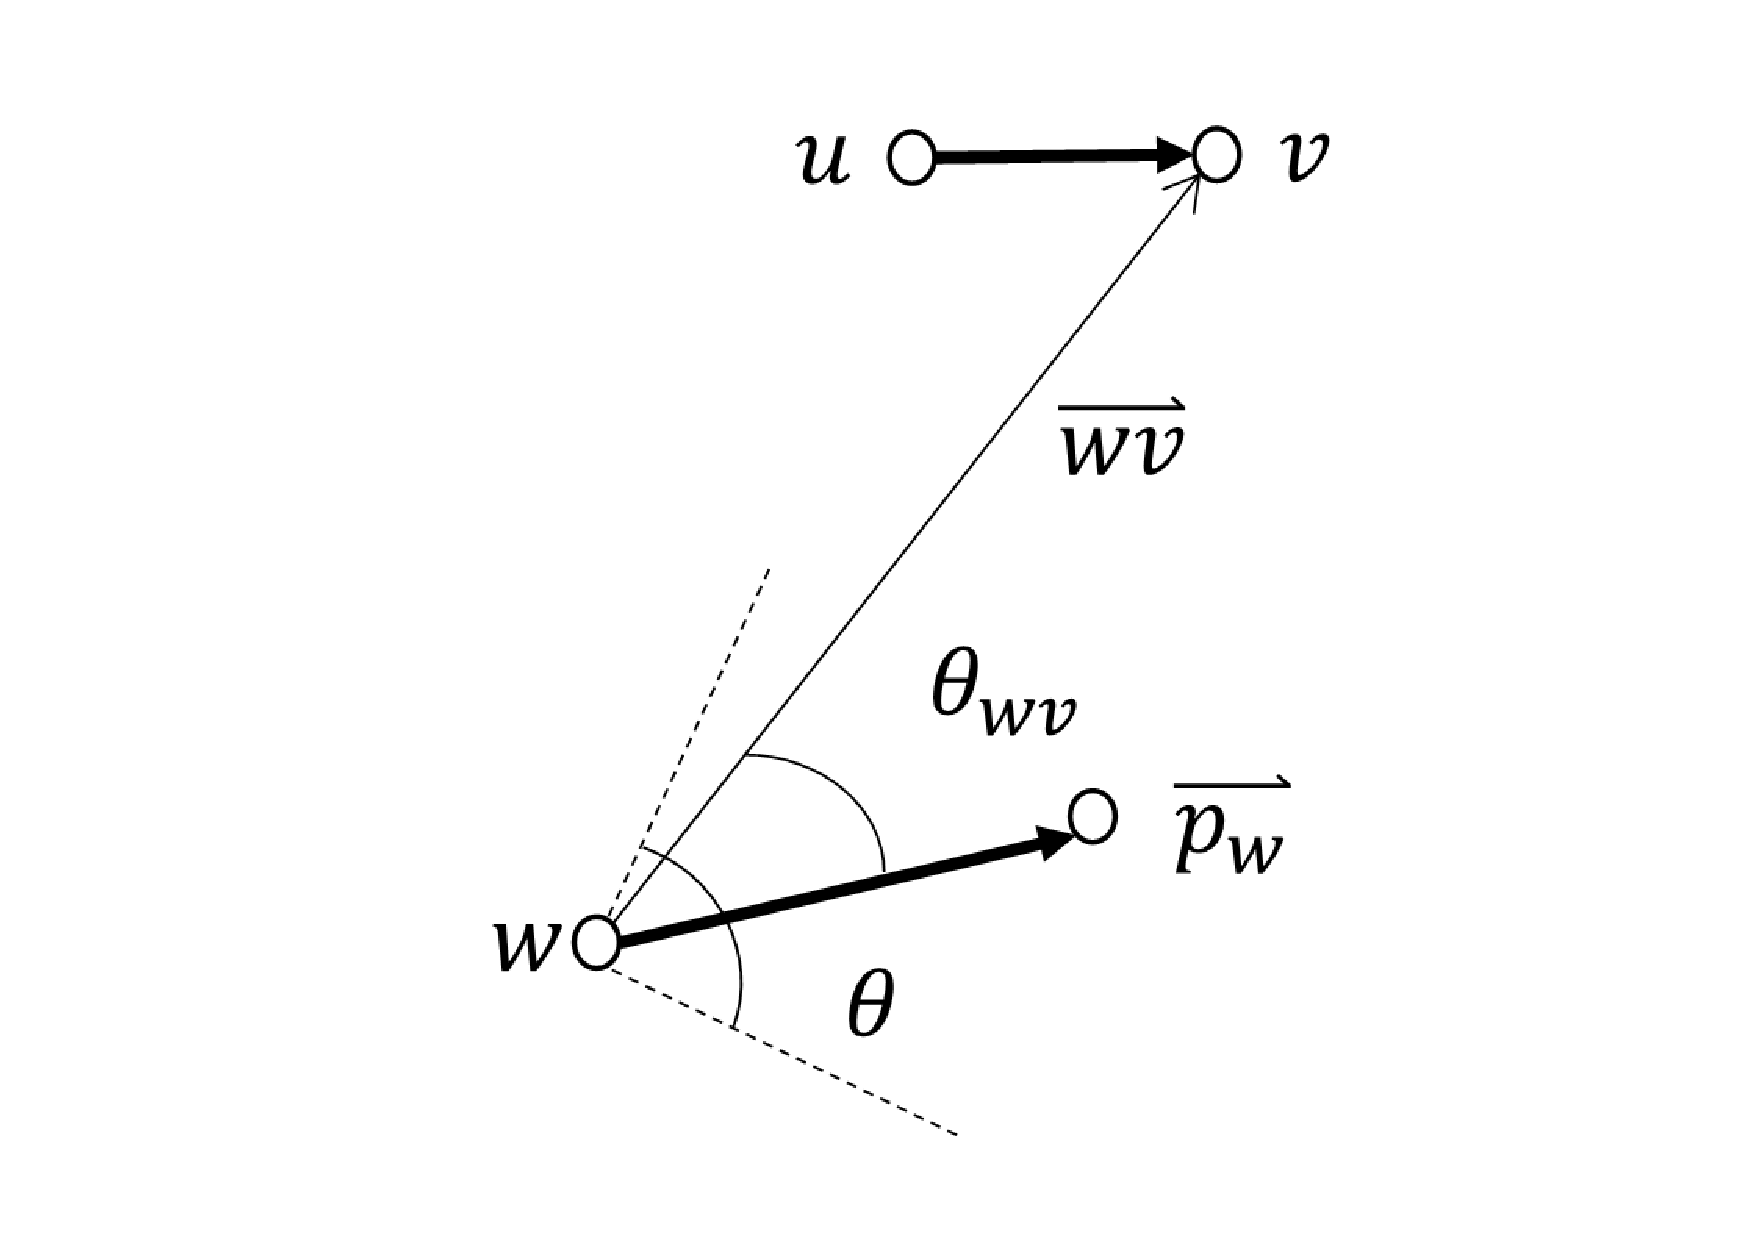
\includegraphics[width=3in]{image/direction.pdf}
% where an .eps filename suffix will be assumed under latex,
% and a .pdf suffix will be assumed for pdflatex; or what has been declared
\DeclareGraphicsExtensions.
\caption{Angle Judge.}
\label{Angle Judge}
\end{figure}

The model was proposed to narrow the interference angle by using directional antenna, so we need to determine whether exist interference between the links that transmission in the same time. Here we use $\varphi _{wv}$ to solve this problem, where vector $\vec {p_w}$ present the send direction of node $w$, the send angle of directional antennas is $\theta _w$. Definition as follows:
\[
\varphi =\left \{ \begin{split}
0 &, \theta_{wv}>\theta_w /2,\\
1 &, \theta_{wv}\leq \theta_w /2,
\end{split}
\right.
\]
where $\theta _{wv}$ is the angle between antenna direction $\vec {p_w}$ of sender node $w$ with the vector $\vec {wv}$ that the direction of sender node $w$ to receiver node $v$. We use this angle to judge whether the receiving node is in the send range of the sender node. As shown in Fig. \ref{Angle Judge}. We can use the following formulate to get the angle $\theta_{wv}$, and decide the interference between links.
\begin{equation*}
  \theta_{wv}=\arccos{(\frac{\vec{p_w} \vec{wv}}{|\vec{p_w}| |\vec{wv}|})}.
\end{equation*}

In this research, we assume that all nodes transmit with the same power level $P$. There are some definition, use $P_{vv}=PG_sG_r/d^{\alpha}_{vv}$ represent the signal receive power of $r_v$ send by $s_v$, and $I_{wv}=P G_{s_w} G_{r_v} \varphi_{wv}/d^{\alpha}_{wv}$ denote the signal interference received by node $r_v$ from a sender $s_v$ that transmit at the same time.


% You must have at least 2 lines in the paragraph with the drop letter
% (should never be an issue)

\section{The Scheduling Algorithm}
In order to solve the scheduling problem of OSML (One-slot Maximum Set of Links), we present the follow OSML algorithm. Start with some definitions, the \emph{relative interference} (RI) of a link $l_u$ on link $l_v$, namely $RI_u(v)=I_{uv}/P_{vv}$. The \emph{affectedness} (proposed in \cite{2}) of link $l_v$, caused by a set of links $S$, is the sum of the relative interferences of the links in $S$ on $l_v$, as well as the effect of noise, scale by $\beta$, or
\begin{equation}
\begin{split}
  A_S(l_v)&=\beta \bigg(\frac{N}{P_{vv}}+\sum _{l_u \in S}RI_u(v)\bigg)\\
  &=\beta \frac{\sum_{l_u \in S}I_{uv}+N}{P_{vv}}.
\end{split}
\end{equation}

The formula of \emph{affectedness} was got from $\textrm{SINR} \geq \beta$. Observe that the \emph{affectedness} of link $l_v$ satisfy $A_S(l_v)\leq 1$, equivalent to the $\textrm{SINR} \geq \beta$, means link $l_v$ can successful transmission.

\begin{algorithm}
\caption{OSML Algorithm}
\label{alg1}
\begin{algorithmic}[1]
\REQUIRE Set of links in the increasing order of length $L={l_1,l_2,...,l_n};$ $S \leftarrow \emptyset,$ $I \leftarrow \emptyset,$ $L_1 \leftarrow \emptyset$.
\ENSURE OMSL schedule $S$.
\STATE Set c according to Eq. (\ref{value of c}).
\REPEAT
\STATE $l_v=(s_v,r_v) \leftarrow$ the first link in $L$.
\STATE $L \leftarrow L \backslash {l_v},$ $S \leftarrow S\cup {l_v}$.
\STATE $L_1 \leftarrow l_u \in L:$ $d(s_u,r_v) \leq c \cdot d_{vv},$ $\varphi_{uv}=1$.
\STATE $L \leftarrow L \backslash L_1$.

\REPEAT
\STATE $l_w \in L \leftarrow$ satisfy $\varphi_{wv}=1$.
\STATE $I \leftarrow I \cup {l_w}$.
\UNTIL{$L$ is traversal end.}

\REPEAT
\STATE $l_a=(s_a,r_a) \leftarrow$ the first link in $I$.
\STATE $I \leftarrow I \backslash l_a$.
\REPEAT
\STATE $I_a \leftarrow l_u \in I:$ $d_{ua}=d(s_u,s_a) \leq  d_{aa}/2$.
\STATE $I \leftarrow I \backslash I_a$.
\STATE $L_v \leftarrow I_a \cup L_2$.
\UNTIL{$I$ is traversal end.}
\UNTIL{$I=\emptyset$. }

\STATE $L \leftarrow L \backslash L_v$.
\STATE Set $I \leftarrow \emptyset$.
\STATE $L_2 \leftarrow l_u \in L:$ $A_S(l_u) \geq 2/3$.
\STATE $L \leftarrow L \backslash L_2$.
\UNTIL{$L=\emptyset$.}
\RETURN $S$.
\end{algorithmic}
\end{algorithm}

Our approximation algorithm for OSML is outlined above. We can simplify the algorithm as a brute-force method. Let $L$ be the set of given communication links, we assume that each link $l_v\in L$ can success communication, added to the solution, its safety ($\textrm{SINR} \geq \beta$) is guaranteed in the step of select. Set $L$ is a sequence which sorted in the increasing order of length of links. Depend on the definition of SINR, we can get the feature that the shorter the length, the more stable of the link. $S$ stores the link in one of independent set, and $I$ is the set of links have interference with the select link $l_v$ in each iterative. In every iteration of the algorithm, there have three step to select the legal and remove illegal link. The first link $l_v$ in $L$ is moved from $L$ to $S$, and use this link as the begin of the first round of selection. The first step (line 6) we need discards all links $l \in I$ whose sender are close to the receiver of $l_v$, meaning $d(r_v,s_w) \leq c \cdot d_{vv}$ ($c$ is a constant bigger than 2, and explained in next part).
\begin{equation}\label{value of c}
c=\max{  \bigg( 2,(2 \cdot 3^3 \cdot \beta \cdot \frac{\alpha-1}{\alpha-2})^{\frac{1}{\alpha-2}}\bigg)}.
\end{equation}
Then make sure the distance between any two links from set $I$ is bigger than $d_{vv}$, remove the illegal links from $L$ (line 16). The last step (line 23), all links $l_u \in L$, whose \emph{affectedness} $A_s(l_u)$ rose to or above a threshold of $2/3$, are removed from $L$ (the number of $2/3$ will explain in next part). This iterative is repeated until all links in $L$ have been select or deleted. In the end, we will get the scheduling set $S$ from OSML algorithm. Next we prove that the obtained schedule is both correct and competitive.



\subsection{Correctness of OSML Algorithm}
In this section we prove that the solution $S$ obtained in OSML Algorithm is correct, all selected links can be scheduled concurrently without collisions, $\forall l_v \in S$, $A_S(l_v) \leq 1$.

There some definitions need to be used in the proof. For link $l_v \in S$, let $S^-_v$ be the set of links that length shorts than $l_v$, and  $S^+_v$ be the links longer than $l_v$, there have some interference between $l_v$ and any link $l_w$ from $S^-_v$ or $S^+_v$ ($\varphi_{wv}=1$).

We can get from third part in iteration of the algorithm (line 22), each link in the scheduling set $S$ satisfy that the \emph{affectedness}, $A_{S^-_v}(l_v) \leq 2/3$, means that for each links $l_v \in S$, when the link is add to the set $S$, the \emph{affectedness} of $l_v$ get by $S^-_v$ is less than $2/3$, since it has not been deleted by in the previous step. In order to ensure that each links in $S$ can be successful communication at the same time slot, the SINR of each link should be satisfy $\textrm{SINR} \geq \beta$. It show that we just need to ensure $\forall l_v \in S $, $ A_{S^+_v}(l_v) \leq 1/3$.

In order to give a clear analyse, here are some geometric definition now. We used $D_w$ present the discs of radius $d_{ww}/2$ around receiver node $s_w \in S^+_v$. From the first elimination criterion, we know the discs $D_w$ do not contain any sender $s_z \neq s_w$ and $s_z \in S^+_v$. Focus on the links set $I$ which have interference on link $l_v$. At the first, division the sender set in $I$ into concentric rings $Ring_k$ which have evenly spaced of $cd_{vv}$ around the receiver $r_v$. Each ring $Ring_k$ contains all senders $s_w \in S^+_v$, for which $k(cd_{vv}) \leq d_{wv} \leq (k+1)(c d_{vv})$. Because of $d_{wv} \geq c \cdot d_{vv}$, so that the first ring $Ring_0$ does not contain any sender from $S^+_v$. Consider all senders $s_w \in Ring_k$, for the concentric rings $Ring_k$, $k>0$. All discs $D_w$ of radius $d_{vv}/2$ around node $s_w$ which located in $Ring_k$ must be completely contained in an extended ring $EXRing_k$, and the area is calculated by the fellow formula:
\begin{equation*}
\begin{split}
A(EXRing_k)&=[(d_{vv}(k+1)c+ d_{vv}/2)^2\\
&   - (d_{vv}kc - d_{vv}/2)^2]\pi  \\
&=c(2k+1) (c+1) d^2_{vv}\pi.
\end{split}
\end{equation*}

Since that each around discs $D_w$ of area $A(D_w) \leq d^2_{vv}\pi/4$ around senders $s_w \in I$ do not intersect, and the minimum distance between $r_v$ and $s_w$ is $k \cdot c \cdot d_{vv}$, $s_w \in Ring_k$, $k>0$. The total interference coming from ring $Ring_k$, $k>1$ is bounded by
\begin{equation*}
\begin{split}
I_{Ring_k}(l_v)&\leq \sum_{s_w \in Ring_k} I_{s_w}(l_v)\\
&\leq \frac{A(EXRing_k)}{A(D_w)}\cdot \frac{PG_{s_w}G_{r_v}\varphi_{wv}}{(kcd_{vv})^{\alpha}}\\
&\leq \frac{4(2k+1)(c+1)c}{k^{\alpha}c^{\alpha}}
\cdot \frac{PG_{s_w}G_{r_v}\varphi_{wv}}{(d_{vv})^{\alpha}}\\
&\leq \frac{1}{k^{\alpha -1}} \cdot \frac{1}{c^{\alpha-2}}
\cdot \frac{PG_{s_w}G_{r_v} \varphi_{wv} }{d^{\alpha}_{vv}} \cdot  3^2 \cdot 2.
\end{split}
\end{equation*}
The value of $PG_{s_w}G_{r_v}\varphi_{wv}$ is fixed in above deduce. $A(EXRing_k)/A (D_w)$ represent the maximum number of links have interference to link $l_v$ in the ring $Ring_k$, and we choose $d(s_w,r_v) =k(cd_{vv})$ ensure the interference to $l_v$ is the maximum. The last inequality holds since $k \geq 1$ and $c \geq 2$, obtain $2k+1 \leq 3k$ and $c+1 \leq 3c/2$. Summing up the interferences over all rings yields
\begin{equation*}
\begin{split}
  I_{S^+_v}(l_v)& < \sum_{k=1,...n} I_{Ring_k}(l_v)\\
  &\leq \sum_{k-1,...n} \frac{1}{k^{\alpha -1}} \cdot \frac{1}{c^{\alpha-2}} \cdot \frac{PG_{s_w}G_{r_v}\varphi_{wv}}{d^{\alpha}{vv}} \cdot 2\cdot3^2  \\
  &<\frac{\alpha -1}{\alpha-2} \cdot \frac{1}{c^{\alpha-2}} \cdot \frac{PG_{s_w}G_{r_v} \varphi_{wv}}{d^{\alpha}_{vv}} \cdot 2 \cdot 3^2,
\end{split}
\end{equation*}
where the last inequality holds since $\alpha >2$. This results in affectedness
\begin{equation*}
\begin{split}
  A_{S^+_v}(l_v) & =\beta \cdot \frac{\sum_{l_u \in S^+_v}RI_u(v)+N}{P_{vv}}\\
 & =\beta \cdot \frac{I_{S^+_v}(l_v)+N}{P_{vv}}\\
 & <\frac{\alpha-1}{\alpha-2} \cdot \frac{2 \cdot 3^2}{c^{\alpha-2}} \cdot \frac{1}{P_{vv}} \cdot \frac{PG_{s_w}G_{r_v} \varphi_{wv}}{d^{\alpha}_{vv}}\\ &+\frac{N \cdot \beta}{P_{vv}}\\
  \end{split}
\end{equation*}

In order to simplify the analysis, assume that there have no ambient noise $N=0$, antennas gain and the sending power of each nodes were fixed value.
\begin{equation}\label{refer C}
\begin{split}
A_{S^+_v}(l_v)=\frac{\alpha-1}{\alpha-2} \cdot \frac{2 \cdot 3^2}{c^{\alpha-2}} \cdot \beta \leq 1/3 \Rightarrow \\
c=\max { \bigg( 2,(2 \cdot 3^3 \cdot \beta \cdot \frac{\alpha-1}{\alpha-2})^{\frac{1}{\alpha-2}}\bigg)}.
\end{split}
\end{equation}

We have shown that each $l_v \in S$, satisfy $A_S(l_v) = A_{S^-_v}(l_v) + A_{S^+_v}(l_v) \leq 2/3 +1/3=1$, which means that $\textrm{SINR} \geq \beta$ for each link in scheduling set $S$. From above mathematical analysis, the value of $c$ was depend on design of third elimination part in algorithm. The judgement of $A_{S^-_v}(l_v) \leq 2/3$ just personal sense, and we proved the correctly.

\subsection{Performance Analysis of OSML Algorithm}
To analyze the performance of algorithm, we compared the solution $ALG$ of OSML algorithm to an optimal solution, say $OPT$. Considering the complexity of directional transmission, we set some special case, and analyse the performance under those case. At first, give some lemma that satisfy the condition of omnidirectional antennas $\theta = 360^{\circ}$.

\emph{lemma 1}: Let $X$ be a feasible solution and let $l_v$ be a link in $X$. The number of sender nodes in $X$ within distance $k \cdot d_{vv}$, $k \geq 1$ of the receiver $r_v$ is at most $k^\alpha$.

\emph{Proof}: The relative interference of each sender $l_u \in X \backslash {l_v}$, where $d_{uv} \leq k \cdot d_{vv}$

\begin{equation*}
  RI_u(v)=\frac{I_{uv}}{P_{vv}}=\frac{P/d^\alpha_{uv}}{P/d^\alpha_{vv}}=(\frac{d_{vv}}{d_{uv}})^\alpha \geq \frac{1}{k^\alpha},
\end{equation*}
which means the maximum number is $k^{\alpha}$, otherwise the $\sum_{l_u \in X} RI_u(v) > 1$. Thus the lemma was been proved.

Then, we set other spacial case that communication angle is $\theta = 180^{\circ}$ of each nodes, and have the same orientation angle. Along with the direction of the orientation angle, the length of links getting shorter and shorter. In this case, the shortest link have no influence to the transmission of other links, which means the last elimination step (line 23) of algorithm have no effect, but get the interference from the larger length of links. $ALG_{180}$ represent the solution of OSML algorithm, and $OPT_{180}$ is the optimal solution in the same condition.

\emph{lemma 2}: In $k$th iteration of the algorithm, we got one link to the solution $ALG_{180}$ and $|OPT_k| \leq (c+(k-1)/2)^{\alpha}$, $OPT_k$ was the optimal solution in $k$th iteration.


\emph{Proof}: Due to the special condition, we just need analyse the first and second elimination part in the algorithm. Consider the set $X_v \subseteq OPT_{180}$ eliminated in the first part of algorithm (line 6), in the iteration when link $l_v \in ALG_{180}$ was added to the scheduling solution. Each link $l_w \in X_v$ is of length at least $d_{vv}$, and the distance of its sender at most $c \cdot d_{vv}$ from receiver $r_v$. By \emph{Lemma 2}, there can be at most $c^{\alpha}$ in the set $X_v$.

For the second part of the proof, which equivalent to a pretreatment for the next iteration of the algorithm. Consider the set $L_v \subseteq L$ that the length of each links bigger than the link $l_v \in ALG_{180}$. In this part of eliminated, ensure the distance of each sender of links at least $d_{vv}/2$. We used the $Y_k$ represent the links which exist in second part of elimination at $k$th iteration, and the $d_k$ is the distance of the $k$th iteration when link $l_k \in ALG_{180}$ added to the scheduling solution, $d_k= d(l_k)/2$.

Combine the result of the last iteration. In the $k$th iteration, it is possible that the links in the discs around $l_w \in Y_k$ was been delete with the radius at most $R_k$. In the first iteration, the radius $R_1 = d_1= d(l_1)/2 \leq d_k$. If $k=2$, $R_2= R_1+ d_2 \leq 2 d_k$. From the induction result, in the $k$th iteration, which $l_v$ added to the solution. At worst, maybe delete all the links in the discs of radius $R_k=R_{k-1} + d_{vv}/2 \leq k \cdot d_{vv}/2$ around each sender $s_w \in Y_k$.

In general, during the process of $k$th iteration, $l_v \in ALG_{180}$ was the legal link. Combine the first part and second part of elimination. Each link $l_w \in X_v$ is of length at least $d_{vv}$ and has its sender of distance at most $c \cdot d_{vv} + (k-1) \cdot d_{vv}/2$ from receiver $r_v$. Therefore, can be at most $(c+(k-1)/2)^{\alpha}$ senders in $X_v$.

Due to the complexity of the directional antennas, we can not offered generally demonstration for the algorithm. But the number of non-intersect links is the least number of scheduling links. In other words, all of the non-intersect links can be scheduling at the same time.

In next section, we will shown the performance of the OSML algorithm.




\section{Evaluations}
In this section, we validate OSML's performance through simulation analysis. We compared the performance with One-slot scheduling algorithm (proposed in \cite{2}). We present the performance of algorithm under the influence of links number, directional antennas interference range and antennas gains.

To simplify the analysis of experiment result. We list the following conditions:
(1) All of the links random distributed on a plane field of size $1000*1000$ units (see Fig. \ref{Simulated Topologies}).
(2) All of the links transmit in the same power.
(3) In the experimental, we ignore the influence by ambient noise $N=0$.

\begin{figure}[htpb]
\centering
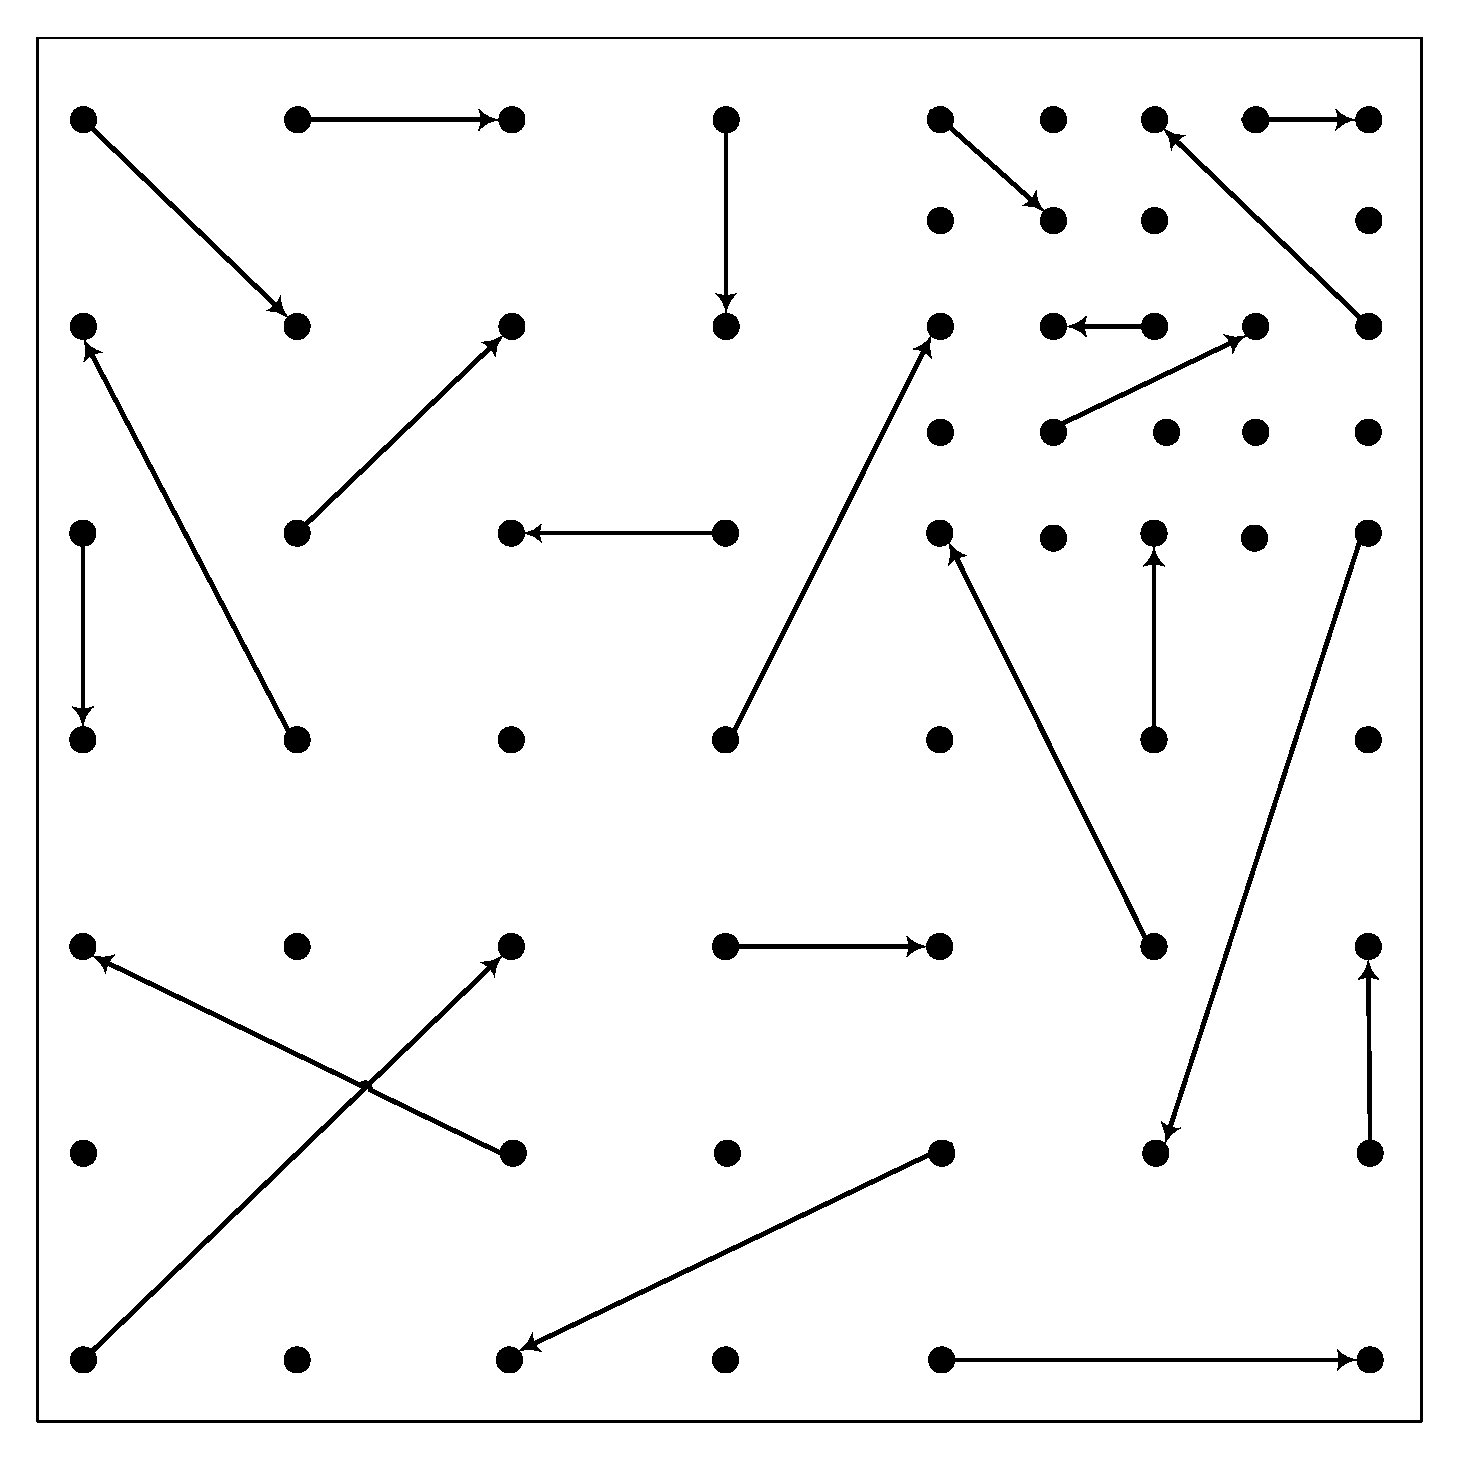
\includegraphics[width=2in]{image/topology.pdf}
% where an .eps filename suffix will be assumed under latex,
% and a .pdf suffix will be assumed for pdflatex; or what has been declared
\DeclareGraphicsExtensions.
\caption{Simulated Topologies.}
\label{Simulated Topologies}
\end{figure}

In OSML scheduling algorithm, The size of the independent set present the performance of the algorithm. In our experiment, we using the number of links of the independent set as the performance standard.

 We give some parameter values used in experiment. Path-loss exponent $\alpha =3$, minimum SINR required for a message to be successfully received $\beta =1.2$, ambient noise $N=0$. Maximum of the link length $l_{max}=20$ and the minimum $l_{min}=10$. General condition, the directional angle of the antennas $\theta =60^{\circ}$, and the antenna gain $Gain=20$.

\subsection{Experimental Results and Analysis}


\begin{figure}[htpb]
\centering
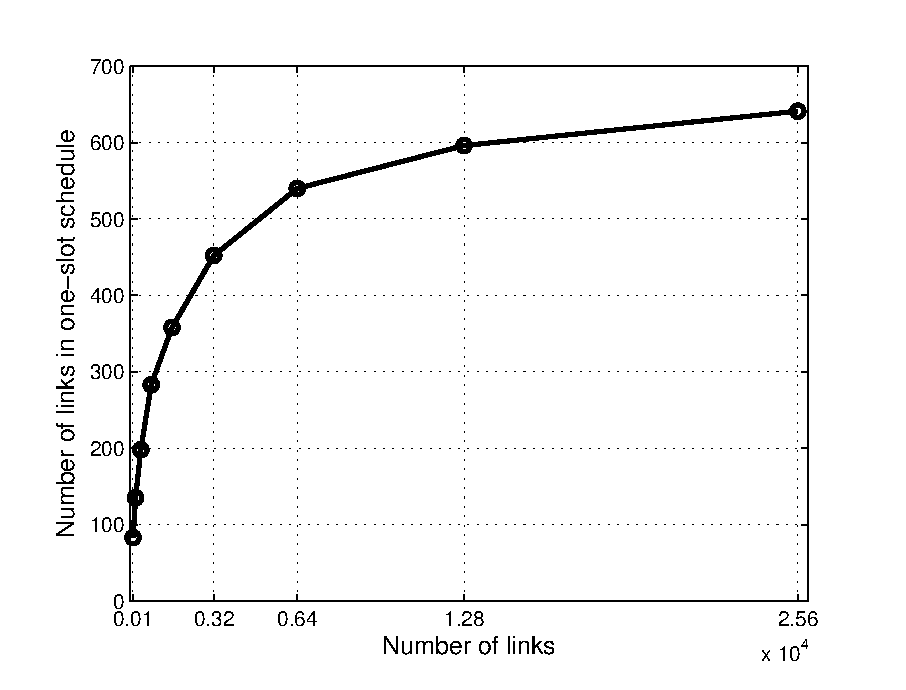
\includegraphics[width=2.5in]{image/1.eps}
% where an .eps filename suffix will be assumed under latex,
% and a .pdf suffix will be assumed for pdflatex; or what has been declared
\DeclareGraphicsExtensions.
\caption{OSML Scheduling Algorithm. Nodes random distribution and $\theta = 60^{\circ} $ or $\theta = 120^{\circ}$, the number of links in one-slot schedule show the perform of the algorithm.}
\label{OSML Scheduling Algorithm.}
\end{figure}

The results are shown in Fig. \ref{OSML Scheduling Algorithm.}, we analyze affect by the length of the input scheduling set to the algorithm, and set $n \in \{100,200,400,800,1600,3200,6400,12800,25600\}$. The simulation present that the size of the maximum independent set grows along with the increase of the number of the request link, but due to the limitations of the space, growth rate becomes slower and tends to balance.

We have a general impression of the performance of the algorithm from above results. Now we give some results from other aspect to the algorithm. First, the influence by the directional angle, the range of the angle satisfied $\theta \in \{30^{\circ},60^{\circ},90^{\circ},...,360^{\circ}\}$, and we make a comparison experiment $n=100$ and $n=3200$. In Fig. \ref{Influence of Directional Angle}. We known that the angle make a great influence to the performance of the OSML scheduling algorithm, when other parameters were fixed. The smaller the angle, the better performance of the algorithm. In the case of maximum angle $\theta = 360^{\circ}$, the algorithm has a worst performance.

\begin{figure}[htpb]
\centering
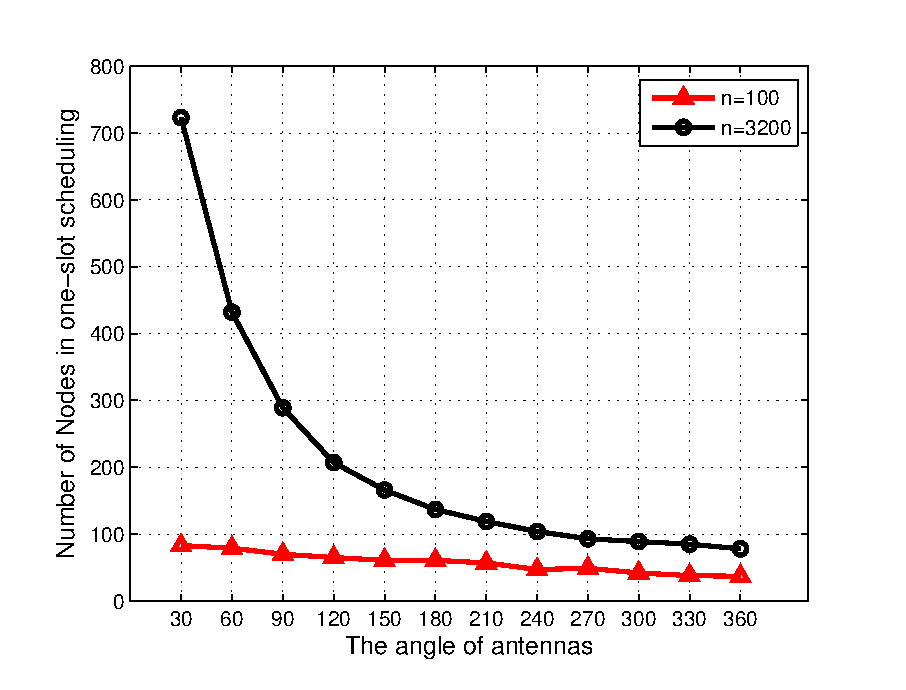
\includegraphics[width=2.5in]{image/3.eps}
% where an .eps filename suffix will be assumed under latex,
% and a .pdf suffix will be assumed for pdflatex; or what has been declared
\DeclareGraphicsExtensions.
\caption{Influence of Directional Angle. Change the angle of the directional antennas, compared the performance in high density with low density.}
\label{Influence of Directional Angle}
\end{figure}

\begin{figure}[!t]
\centering
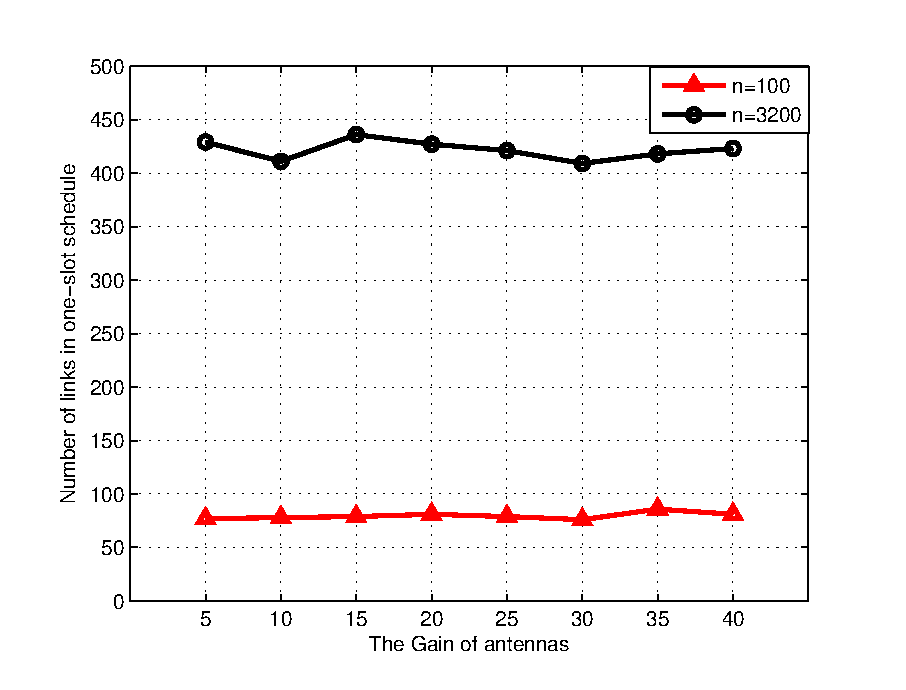
\includegraphics[width=2.5in]{image/4.eps}
% where an .eps filename suffix will be assumed under latex,
% and a .pdf suffix will be assumed for pdflatex; or what has been declared
\DeclareGraphicsExtensions.
\caption{Influence of Antenna Gain. Change the gain of the directional antennas, compared the performance in high density with low density.}
\label{Influence of Antenna Gain}
\end{figure}

Figure \ref{Influence of Antenna Gain} show the results of the influence to the algorithm by the antenna gain. We set up a fixed directional angle $\theta=60^{\circ}$, antenna gain $G \in \{5,10,15,20,25,30,35,40\}$, adopt double groups $n=100$, $n=3200$. According to the formula of SINR, we known that the changes of the antennas gain have a small effect to the result of algorithm. The simulation results shown that even if there have some fluctuation, the antennas gain have limited impact to the algorithm.

The above results were just get by separate analyzed of the OSML algorithm. Now we do some comparison between OSML algorithm and the one-slot scheduling algorithm. Parameter settings: $Gain=20$, $\theta =60^{\circ}$, and the number of links $n \in \{100,200,400,800,1600,3200,6400,12800,25600\}$. Shown in Fig. \ref{Comparison between OSML and One-slot Algorithm 1}, in random network topology, the performance of the OSML algorithm is batter than the one-slot algorithm. This is advantage of directional antennas, reduce the interference range by every nodes. In a fixed range of scene, more link can be allow for transmit together. In Fig. \ref{Comparison between OSML and One-slot Algorithm 2}, we change the angle of the antenna $\theta=360^{\circ}$, two curves of the algorithm are very similar in the condition of lower density, but slightly worse than one-slot algorithm in high density network. This performance is the comparison of the algorithm. OSML was designed to adapt the situation of direction. So the OSML has limited performance than other omnidirectional algorithm.

\begin{figure}[!t]
\centering
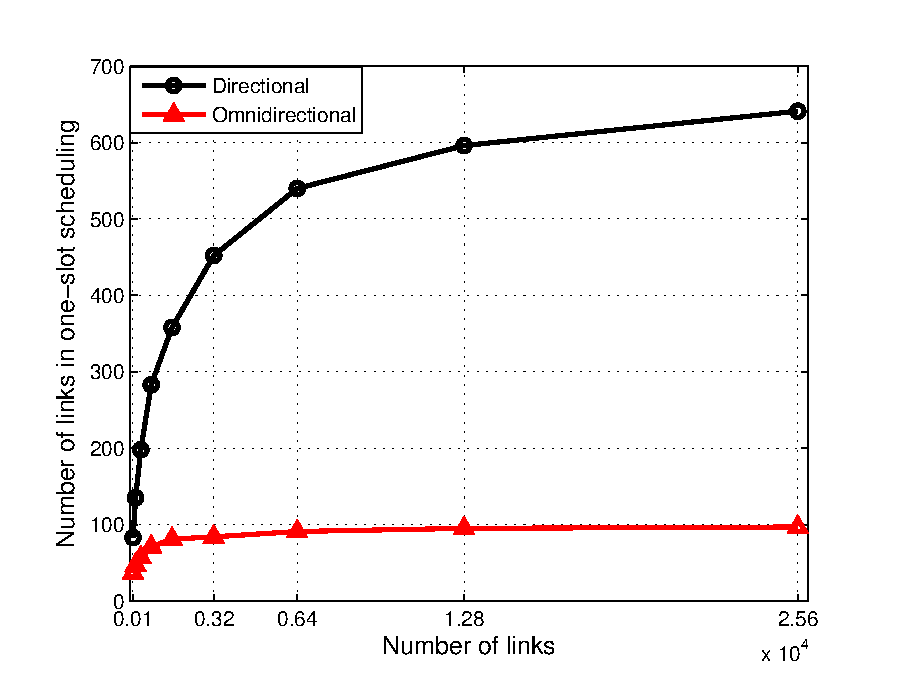
\includegraphics[width=2.5in]{image/5.eps}
% where an .eps filename suffix will be assumed under latex,
% and a .pdf suffix will be assumed for pdflatex; or what has been declared
\DeclareGraphicsExtensions.
\caption{Comparison between OSML and One-slot Algorithm. Use the same simulation data which generated at randomly by computer, but add the parameter of directional angle $\theta=60^{\circ}$ or $\theta=120^{\circ}$ when use to running OSML algorithm.}
\label{Comparison between OSML and One-slot Algorithm 1}
\end{figure}


To sum up, in random distribution wireless network, it has get an obvious effect to reduce the interference when multiple links transmission simultaneously by using directional antennas. The OSML scheduling algorithm have better performance than this omnidirectional algorithm, and we also obtain that the antenna gain have a limited effect to the algorithm, but seriously influence by directional angle.

\begin{figure}[!t]
\centering
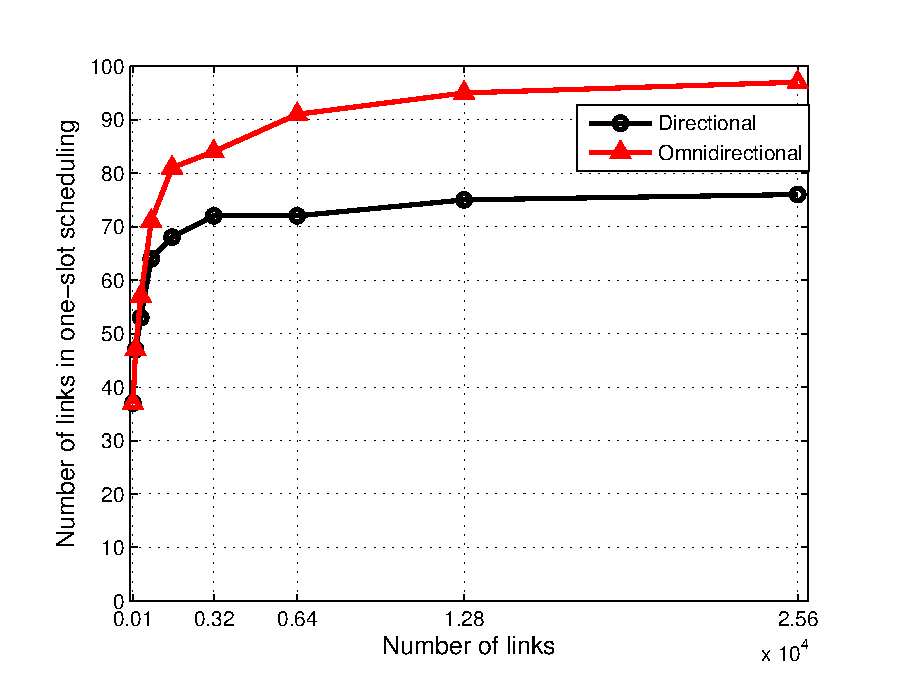
\includegraphics[width=2.5in]{image/6.eps}
% where an .eps filename suffix will be assumed under latex,
% and a .pdf suffix will be assumed for pdflatex; or what has been declared
\DeclareGraphicsExtensions.
\caption{Comparison between OSML and One-slot Algorithm. Set the directional angle $\theta=360^{\circ}$, which means use same random data running in different algorithm, compared the performance of two algorithm.}
\label{Comparison between OSML and One-slot Algorithm 2}
\end{figure}
% An example of a floating figure using the graphicx package.
% Note that \label must occur AFTER (or within) \caption.
% For figures, \caption should occur after the \includegraphics.
% Note that IEEEtran v1.7 and later has special internal code that
% is designed to preserve the operation of \label within \caption
% even when the captionsoff option is in effect. However, because
% of issues like this, it may be the safest practice to put all your
% \label just after \caption rather than within \caption{}.
%
% Reminder: the "draftcls" or "draftclsnofoot", not "draft", class
% option should be used if it is desired that the figures are to be
% displayed while in draft mode.
%
%\begin{figure}[!t]
%\centering
%\includegraphics[width=2.5in]{myfigure}
% where an .eps filename suffix will be assumed under latex,
% and a .pdf suffix will be assumed for pdflatex; or what has been declared
% via \DeclareGraphicsExtensions.
%\caption{Simulation Results.}
%\label{fig_sim}
%\end{figure}

% Note that IEEE typically puts floats only at the top, even when this
% results in a large percentage of a column being occupied by floats.


% An example of a double column floating figure using two subfigures.
% (The subfig.sty package must be loaded for this to work.)
% The subfigure \label commands are set within each subfloat command,
% and the \label for the overall figure must come after \caption.
% \hfil is used as a separator to get equal spacing.
% Watch out that the combined width of all the subfigures on a
% line do not exceed the text width or a line break will occur.
%
%\begin{figure*}[!t]
%\centering
%\subfloat[Case I]{\includegraphics[width=2.5in]{box}%
%\label{fig_first_case}}
%\hfil
%\subfloat[Case II]{\includegraphics[width=2.5in]{box}%
%\label{fig_second_case}}
%\caption{Simulation results.}
%\label{fig_sim}
%\end{figure*}
%
% Note that often IEEE papers with subfigures do not employ subfigure
% captions (using the optional argument to \subfloat[]), but instead will
% reference/describe all of them (a), (b), etc., within the main caption.


% An example of a floating table. Note that, for IEEE style tables, the
% \caption command should come BEFORE the table. Table text will default to
% \footnotesize as IEEE normally uses this smaller font for tables.
% The \label must come after \caption as always.
%
%\begin{table}[!t]
%% increase table row spacing, adjust to taste
%\renewcommand{\arraystretch}{1.3}
% if using array.sty, it might be a good idea to tweak the value of
% \extrarowheight as needed to properly center the text within the cells
%\caption{An Example of a Table}
%\label{table_example}
%\centering
%% Some packages, such as MDW tools, offer better commands for making tables
%% than the plain LaTeX2e tabular which is used here.
%\begin{tabular}{|c||c|}
%\hline
%One & Two\\
%\hline
%Three & Four\\
%\hline
%\end{tabular}
%\end{table}


% Note that IEEE does not put floats in the very first column - or typically
% anywhere on the first page for that matter. Also, in-text middle ("here")
% positioning is not used. Most IEEE journals/conferences use top floats
% exclusively. Note that, LaTeX2e, unlike IEEE journals/conferences, places
% footnotes above bottom floats. This can be corrected via the \fnbelowfloat
% command of the stfloats package.



\section{Conclusions}

 In this paper, we developed a directional interference model for wireless network where the nodes using directional antennas. We first proposed a OSML approximation algorithm based on the directional interference model, and show the performance by simulation and mathematical analysis. The results of experiments proved that the performance of OSML was greatly affected by antenna interference angle, but not sensitive to antenna gains. Compared with the omni-directional antennas algorithm, OSML bring better result due to the nature of directional antennas. However, there are several challenges to OSML. The radiation beam of directional antenna is more complicated than we thought. From the OSML algorithm, we show the advantage of directional antenna to the problem of link scheduling, and hope that will be a significant step to solve this problem.

% conference papers do not normally have an appendix


% use section* for acknowledgement
%\section*{Acknowledgment}
\section*{Acknowledgments}
\indent This work was supported by Natural Science Foundation of China under Grants No.~61202442, NO.~61502075 and NO.~61272524.



\bibliographystyle{IEEEtran}

\bibliography{IEEEabrv,RTDA}






% that's all folks
\end{document}


